\begin{figure}
    \centering
    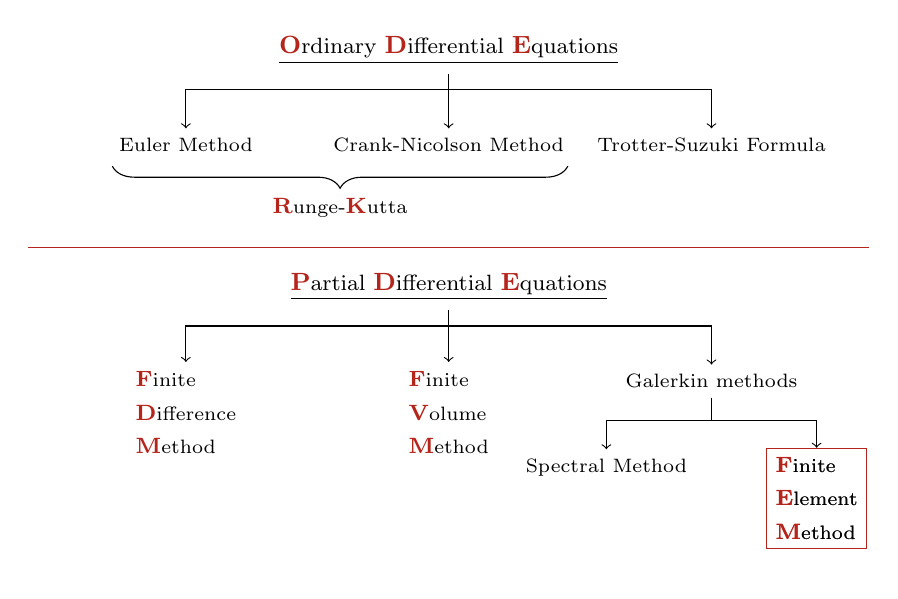
\begin{tikzpicture}[x=0.89cm]

        \node[align=left] at (0,5) (A) {\underline{\small{\textbf{\textcolor{BrickRed}{O}}}\footnotesize{rdinary }\small{\textbf{\textcolor{BrickRed}{D}}}\footnotesize{ifferential }\small{\textbf{\textcolor{BrickRed}{E}}}\footnotesize{quations}}};

        \node at (0,3.8) (B) {\scriptsize{Crank-Nicolson Method}};

        \node at (-3.75,3.8) (C) {\scriptsize{Euler Method}};

        \node at (3.75,3.8) (D) {\scriptsize{Trotter-Suzuki Formula}};

        \draw[->] (A) -- (B);
        \draw[->] (0,4.5) -- (-3.75,4.5) -- (C);
        \draw[->] (0,4.5) -- (3.75,4.5) -- (D);

        \draw[decorate, decoration={brace, amplitude=8pt, raise=2pt}] (1.7,3.6) -- (-4.8,3.6);
        \node at (-1.55,3) (E) {\footnotesize{\textbf{\textcolor{BrickRed}{R}}}\scriptsize{unge-}\footnotesize{\textbf{\textcolor{BrickRed}{K}}}\scriptsize{utta}};

         

        \draw[BrickRed] (-6,2.5) -- (6,2.5);



        \node[align=left] at (0,2) (F) {\underline{\small{\textbf{\textcolor{BrickRed}{P}}}\footnotesize{artial }\small{\textbf{\textcolor{BrickRed}{D}}}\footnotesize{ifferential }\small{\textbf{\textcolor{BrickRed}{E}}}\footnotesize{quations}}};

        \node[align=left] at (0,0.4) (G) {\footnotesize{\textbf{\textcolor{BrickRed}{F}}}\scriptsize{inite}\\\footnotesize{\textbf{\textcolor{BrickRed}{V}}}\scriptsize{olume}\\\footnotesize{\textbf{\textcolor{BrickRed}{M}}}\scriptsize{ethod}};

        \node[align=left] at (-3.75,0.4) (H) {\footnotesize{\textbf{\textcolor{BrickRed}{F}}}\scriptsize{inite}\\\footnotesize{\textbf{\textcolor{BrickRed}{D}}}\scriptsize{ifference}\\\footnotesize{\textbf{\textcolor{BrickRed}{M}}}\scriptsize{ethod}};

        \node at (3.75,0.8) (I) {\scriptsize{Galerkin methods}};

        \node at (2.25,-0.3) (J) {\scriptsize{Spectral Method}};

        \node<1>[align=left] at (5.25,-0.69) (Ktext) {\footnotesize{\textbf{\textcolor{BrickRed}{F}}}\scriptsize{\textcolor{black}{inite}}\\\footnotesize{\textbf{\textcolor{BrickRed}{E}}}\scriptsize{\textcolor{black}{lement}}\\\footnotesize{\textbf{\textcolor{BrickRed}{M}}}\scriptsize{\textcolor{black}{ethod}}};

        \node<2->[draw,BrickRed,align=left] at (5.25,-0.69) (K) {\footnotesize{\textbf{\textcolor{BrickRed}{F}}}\scriptsize{\textcolor{black}{inite}}\\\footnotesize{\textbf{\textcolor{BrickRed}{E}}}\scriptsize{\textcolor{black}{lement}}\\\footnotesize{\textbf{\textcolor{BrickRed}{M}}}\scriptsize{\textcolor{black}{ethod}}};

        \draw[->] (F) -- (G);
        \draw[->] (0,1.5) -- (-3.75,1.5) -- (H);
        \draw[->] (0,1.5) -- (3.75,1.5) -- (I);
        \draw[->] (I) -- (3.75,0.3) -- (2.25,0.3) -- (J);
        \draw[->] (I) -- (3.75,0.3) -- (5.25,0.3) -- (Ktext);



        \draw[white] (0,-1.6) -- (0,-1.5);
    \end{tikzpicture}
\end{figure}